\chapter{Goals of the IO-SEA project}\label{chap:goals}
%%{\color{blue} Located in {\ttfamily Goals.tex}}\\

This chapter is an overview of the ambition of the IO-SEA project as presented and exposed in the proposal.
This view is more than three years old. It highlights the main topics that drove the development of the IO-SEA
software stack. We should first quickly summarize them. 

\paragraph{}
Let's take a few seconds and have a look at the backmirror. The very first paragraph of the IO-SEA proposal 
clearly states the ambitions and goals of the project, which are described at this:

\begin{quotation}
IO-SEA aims to provide a novel data management and storage platform for exascale computing based on hierarchical
storage management (HSM) and on-demand provisioning of storage services. The platform will efficiently make use
of storage tiers spanning NVMe and NVRAM at the top all the way down to least active data stored with tape-based
technologies. System requirements are driven by data intensive use-cases, in a very strict co-design approach.
The concept of ephemeral data nodes and data accessors is introduced that allows users to flexibly operate the
system, using various well-known data access paradigms, such as POSIX namespaces, S3/Swift Interfaces, MPI-IO 
and other middleware, data formats and protocols. These ephemeral resources eliminate the problem of treating
storage resources as static and unchanging system components – which is not a tenable proposition for data
intensive exascale environments. The methods and techniques are applicable to exascale class data intensive
applications and workflows that need to be deployed in highly heterogeneous computing environments.
\end{quotation}

\section{Highlights from the proposal}
In this section, we'll shortly remind the technological choices made in IO-SEA, as well as the underlying
concepts that drove the development of IO-SEA. 

\paragraph{}
The proposal then states which technologies and technical approaches to be fostered and leveraged:
\begin{itemize}
    \item object stores
    \item Hierarchical Storage Management (HSM)
    \item ephemeral services and scheduling
    \item IO Instrumentation and AI based analytics
    \item Co-design (this approach was later described by the deliverabmes from Work Package~\#1\cite{iosea-d1.1})
\end{itemize}

\paragraph{}
By taking in considerations those technologies, concepts and topcis to be advanced are then chosen:
\begin{itemize}
    \item Manage system scalability
    \item Manage data scalability
    \item Manage data heterogeneity
    \item Manage Data placement
\end{itemize}

\paragraph{}
In order to build an exascale IO software stack, the work done in IO-SEA was designed to be made following
those tracks:
\begin{itemize}
    \item as filesystem paradigm do not fit the scalability requirements and constraints from the Exascale era.
    The decided choice is to use object stores instead, as they do scale very well. This feature is achieved 
    due to the \textbf{C}reate \textbf{R}ead \textbf{U}pdate \textbf{D}elete (CRUD) semantics, which is simple 
    and compact. Because this semantics is very far from POSIX, which is much more complex, it is required to 
    build pieces of software, based on well identified design concepts. IO-SEA will develop those needed tools, 
    based on two mains ideas, which are \textit{datasets} and \textit{namespaces}. 
    
    \item Tapes is clearly the less expansive technology to be used to store data, making it to save money and 
    power. As IO-SEA has the ambition to manage tens or even hundreds of exabytes of data, using tapes can't
    reasonably be ignored, they clearly are to be used. Tapes have high capacity but they are really slow,
    especially when compared to modern storage media. As IO-SEA will involve HSM mechanisms, tapes are clearly
    a target for integrating this technology.
    
    \item High speed storage, including NVRAM and NVMe capable devices are at the oppositce side ofg the HSM 
    spectrum. As tapes are slow but offer high capacity, and are rather inexpensive, high speed storage is greedy
    in terms of energy consumption and are very expensive, and they do offer a very high bandwidth, a very small
    latency, as the cost of a reduced storage capability. As more classical storage, like rotating HDDs or
    standard SSDs, are inserted in this "storage spectrum", the question of comprehensive management of all
    devices, via an extended HSM implementation, becomes crucial.
    
    \item In order to perform an efficient HSM, it is necessary to collect information in order to have a 
    precise idea about the files to be managed. The first natural source for such information is naturally
    the end-user, who can add tags (or \textit{hints}) in order to help characterizing the pieces of data. Such
    information may be lacking, imprecise or erroneous. It could be necessary, most of the times, to automatize
    this process. In the IO-SEA software, tools are developed and/or leveraged in order to perform an as
    comprehensive as possible collection of information about the different pieces of data. The result of this
    precise IO instrumentation is then post-processed by AI analytics. This recommendation system automatically
    does the job of tagging the files with the correct related tags or hints. Those hints are required to 
    optimize the way the HSM is working and its efficiency. 
    
    \item as new data model are introduced, via HSM and object stores relying on datasets and namespaces 
    meta-structures, and as specific interfaces are developed (like ephemeral services), it makes sense to 
    look forward for new storage access paradigms. Within IO-SEA, the concept of Data and Access Storage 
    Interface (DASI) is introduced.  DASI will encourage applications to describe their data using meaningful semantics, on the one hand facilitating exploitation of those data, and on the other hand giving the opportunity for IO-SEA to optimise data placement given the intended access patterns.
    
    \item a direct consequence of the introduction of the concepts of datasets and namespaces are data nodes ans
    ephemeral services. As storage resourcves as clearly not infinite, batch environments today should schedule the usage of storage capacity and bandwidth. Ephemeral services, running on dedicated data nodes, themselves 
    closely acquainted with some compuofte nodes are introduced. Ephemeral servers may have different kinds or 
    flavors. They are IO server, spawned on demand and associated to a set of compute jobs, are working as
    dedicated IO servers for those compute jobs. It works both as an IO proxy server and as a bridge capable of
    translating the underlying object stores semantics to a different IO semantics. 
\end{itemize}

\paragraph{}
As a raw summary, the different aspects and features of the IO-SEA project may be gathered and
summarized under this schema depicted on the figure \ref{fig:iosea-nutshell} below. 
\begin{figure}[ht]
    \centering
    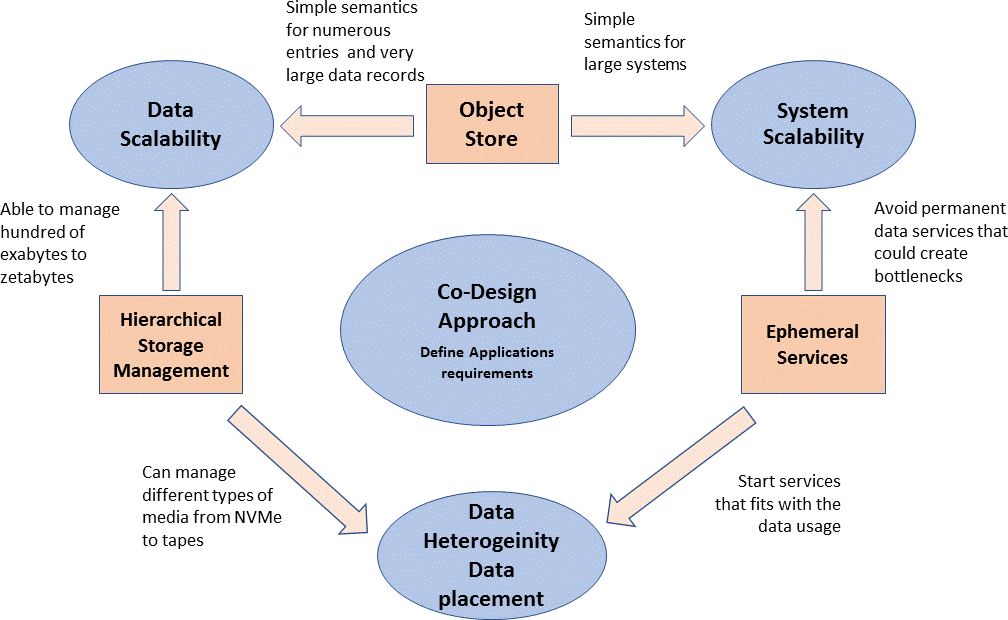
\includegraphics[width=\textwidth]{FIGS/IOsea.png}
    \caption[IO-SEA in a nutshell]{ How the technical choices and the technical challenges interact}
    \label{fig:iosea-nutshell}
\end{figure}

One the fundamental concept and underlying idea of IO-SEA is simple : storage is not an infinite resource, 
from both the capability or bandwidth point of view.   Sharing a restricted resource across a pool of users is
not a new problem and it has already been solved for sharing processors by batch schedulers like Slurm. In order
to use such resource managers, we will introduce two ideas to also handle storage as a shared resource:
\begin{itemize}
    \item Data accessors / ephemeral data services: data accessors are services that provide access to data for applications. For example, it can be a S3 or Swift server exposing objects, or a NFSv4 server that will show a namespace whose files will be connected to objects. Data accessors run as ephemeral services: a simulation workflow is associated with several data accessors; they are spawned at the beginning of the workflow and are dedicated to it. The ephemeral service will have no other clients than those running the simulation applications, and it will end when the workflow ends.
    
    \item Data nodes: ephemeral services need hardware to run on, those nodes are called ‘data nodes’. They have affinities with simulation nodes, which helps the resource manager choose data nodes that are close enough to compute nodes in terms of network location. Data nodes are a resource of the supercomputer, like compute nodes, and as such must be managed by a resource manager.
\end{itemize}

\section{IO-SEA, the MSA and the SEA legacy}

IO-SEA is not a standalone project, it is part of the "SEA legacy", a group of three projects funded under the
same EuroHPC JU call. The three projects target the Exascale era: the DEEP-SEA develops HPC middle-ware and
software, RED-SEA develops a new hardware and software network architecture while IO-SEA provides new storage
paradigm. All the projects go together and have strong interactions.

\begin{figure}[ht]
    \centering
    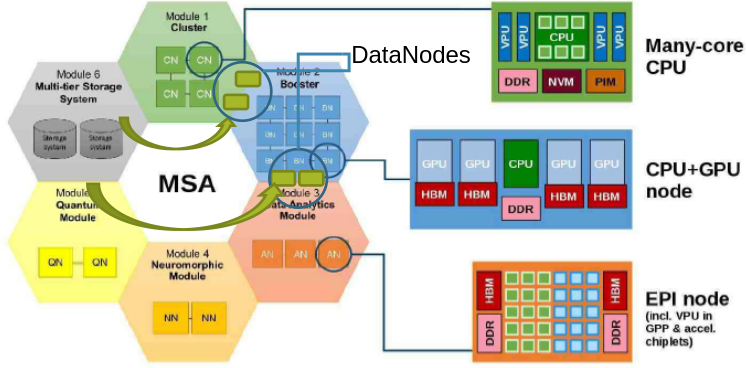
\includegraphics[width=\textwidth]{FIGS/MSA.png}
    \caption[The Modular Supercomputer Architecture]{ Data Nodes and Ephemeral Services within the MSA}
    \label{fig:msa}
\end{figure}

\paragraph{}
At the very core of this strong collaboration relies the Modular Supercomputing Architecture (MSA). MSA is made
of building blocks, or modules, each module having its own specific resources (for example GPU, or neuromorphic
processors). In this scope, it's quite natural to define a "IO module" which will hosts the IO-SEA data nodes
and run most of the server side IO-SEA software stack. With this approach, IO-SEA fits in the MSA as defined 
in figure \ref{fig:msa} . 


\section{The IO-SEA software components and their relationships}

This section describes how the different components of the IO-SEA infrastructure interact. The core of IO-SEA is
made of two object stores. Originally those object stores were the MOTR object store from Seagate, and Phobos an
open-source object store developed at CEA. The big picture of the IO-SEA software stack is described by figure
\ref{fig:iosea-sw-stack}. 

\begin{figure}[ht]
    \centering
    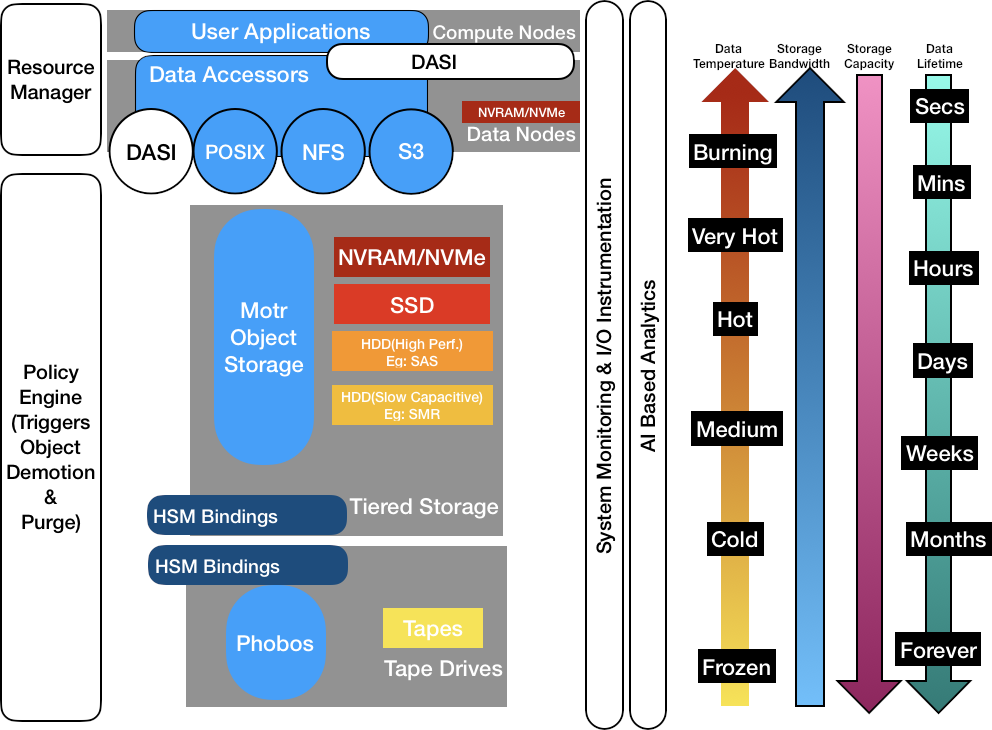
\includegraphics[width=\textwidth]{FIGS/iosea-swstack.png}
    \caption[IO-SEA software stack]{ The components of the IO-SEA software stack}
    \label{fig:iosea-sw-stack}
\end{figure}

Phobos is capable of dealing with tapes. MOTR is capable of dealing with a tiered storage stack, with
different kinds of disks. MOTR is HSM-ready (this is a direct outcome from the SAGE project). Those two object
stores inter-operates via a specifically designed HSM interface. In the run of the IO-SEA project, this component
gave birth to the HESTIA component, with a new and well defined API for HSM management.

\paragraph{}
On top of those HSM connected object stores, advanced interfaces are required, for object stores have very 
simple semantics\footnote{In particular, this makes it possible to scale object store very well}. For the 
majority of use cases, other interfaces are required to implement. For example, POSIX or NFS semantics are to 
be implemented. Dedicated servers are required, those are the ephemeral services. Original ephemeral services as
described in the original proposal includes NFS interface, Burst Buffers with POSIX interface, and S3 interface.
Ephemeral services offer this kind of feature, acting as "bridges" between the objects store semantics (typically
the CRUD semantics) and more complex semantics (like filesystem semantics offered by POSIX or NFS). 

\paragraph{}
Interacting with elaborated middleware, such as those involved and developed in the scope of the DEEP-SEA 
project, is very important. This approach as lead to the design of the Data Access Storage Interface (DASI).

DASI helps the user defining a way to address his scientific data. The user can so define elements composing a 
key that can be use to efficiently addressed the scientific data, with full compliance to the research domain. 
The DASI will then organise the data in a smart way, making all the necessary actions to have this storage
using correctly the object stores and the HESTIA interface. 

DASI will help in implementing other pieces of middle-ware, and may be accelerated by dedicated agents, to be
used as ephemeral services. 

\paragraph{}
Ephemeral services are designed to be attached to some computes jobs: they are dedicated to a compute job or a
set of compute jobs logically chained together. An ephemeral service are strongly associated with their clients
and serve only those clients, on the other side, the clients (the compute jobs) will \textbf{only} do IO via
the ephemeral services. As the compute job starts, the related ephemeral server starts as well, and when the 
compute job ends, the data and metadata are flushed to the object store and the ephemeral service is stopped.

In order to run ephemeral servers, dedicated machines are required. Those machines are called \textit{data nodes}
and should be clearly identified. As seen above, and as shown in figure \ref{fig:msa}, they are grouped into
a specific module with the MSA. 

\paragraph{}
Dedicated software is required to manage the association between the ephemeral services and the compute jobs. 
This lead to the development of the workflow management.

On the other hand, a Policy Engine is needed to manage the data movement between the different level in the
tiered storage stack. The Robinhood software, developed at CEA, was used and modified to deal with this feature.

